\documentclass[]{article}
\usepackage{lmodern}
\usepackage{amssymb,amsmath}
\usepackage{ifxetex,ifluatex}
\usepackage{fixltx2e} % provides \textsubscript
\ifnum 0\ifxetex 1\fi\ifluatex 1\fi=0 % if pdftex
  \usepackage[T1]{fontenc}
  \usepackage[utf8]{inputenc}
\else % if luatex or xelatex
  \ifxetex
    \usepackage{mathspec}
  \else
    \usepackage{fontspec}
  \fi
  \defaultfontfeatures{Ligatures=TeX,Scale=MatchLowercase}
\fi
% use upquote if available, for straight quotes in verbatim environments
\IfFileExists{upquote.sty}{\usepackage{upquote}}{}
% use microtype if available
\IfFileExists{microtype.sty}{%
\usepackage{microtype}
\UseMicrotypeSet[protrusion]{basicmath} % disable protrusion for tt fonts
}{}
\usepackage[margin=1in]{geometry}
\usepackage{hyperref}
\hypersetup{unicode=true,
            pdftitle={Teoría de probabilidad},
            pdfauthor={Martín Andrés Macías Quintero},
            pdfborder={0 0 0},
            breaklinks=true}
\urlstyle{same}  % don't use monospace font for urls
\usepackage{color}
\usepackage{fancyvrb}
\newcommand{\VerbBar}{|}
\newcommand{\VERB}{\Verb[commandchars=\\\{\}]}
\DefineVerbatimEnvironment{Highlighting}{Verbatim}{commandchars=\\\{\}}
% Add ',fontsize=\small' for more characters per line
\usepackage{framed}
\definecolor{shadecolor}{RGB}{248,248,248}
\newenvironment{Shaded}{\begin{snugshade}}{\end{snugshade}}
\newcommand{\KeywordTok}[1]{\textcolor[rgb]{0.13,0.29,0.53}{\textbf{#1}}}
\newcommand{\DataTypeTok}[1]{\textcolor[rgb]{0.13,0.29,0.53}{#1}}
\newcommand{\DecValTok}[1]{\textcolor[rgb]{0.00,0.00,0.81}{#1}}
\newcommand{\BaseNTok}[1]{\textcolor[rgb]{0.00,0.00,0.81}{#1}}
\newcommand{\FloatTok}[1]{\textcolor[rgb]{0.00,0.00,0.81}{#1}}
\newcommand{\ConstantTok}[1]{\textcolor[rgb]{0.00,0.00,0.00}{#1}}
\newcommand{\CharTok}[1]{\textcolor[rgb]{0.31,0.60,0.02}{#1}}
\newcommand{\SpecialCharTok}[1]{\textcolor[rgb]{0.00,0.00,0.00}{#1}}
\newcommand{\StringTok}[1]{\textcolor[rgb]{0.31,0.60,0.02}{#1}}
\newcommand{\VerbatimStringTok}[1]{\textcolor[rgb]{0.31,0.60,0.02}{#1}}
\newcommand{\SpecialStringTok}[1]{\textcolor[rgb]{0.31,0.60,0.02}{#1}}
\newcommand{\ImportTok}[1]{#1}
\newcommand{\CommentTok}[1]{\textcolor[rgb]{0.56,0.35,0.01}{\textit{#1}}}
\newcommand{\DocumentationTok}[1]{\textcolor[rgb]{0.56,0.35,0.01}{\textbf{\textit{#1}}}}
\newcommand{\AnnotationTok}[1]{\textcolor[rgb]{0.56,0.35,0.01}{\textbf{\textit{#1}}}}
\newcommand{\CommentVarTok}[1]{\textcolor[rgb]{0.56,0.35,0.01}{\textbf{\textit{#1}}}}
\newcommand{\OtherTok}[1]{\textcolor[rgb]{0.56,0.35,0.01}{#1}}
\newcommand{\FunctionTok}[1]{\textcolor[rgb]{0.00,0.00,0.00}{#1}}
\newcommand{\VariableTok}[1]{\textcolor[rgb]{0.00,0.00,0.00}{#1}}
\newcommand{\ControlFlowTok}[1]{\textcolor[rgb]{0.13,0.29,0.53}{\textbf{#1}}}
\newcommand{\OperatorTok}[1]{\textcolor[rgb]{0.81,0.36,0.00}{\textbf{#1}}}
\newcommand{\BuiltInTok}[1]{#1}
\newcommand{\ExtensionTok}[1]{#1}
\newcommand{\PreprocessorTok}[1]{\textcolor[rgb]{0.56,0.35,0.01}{\textit{#1}}}
\newcommand{\AttributeTok}[1]{\textcolor[rgb]{0.77,0.63,0.00}{#1}}
\newcommand{\RegionMarkerTok}[1]{#1}
\newcommand{\InformationTok}[1]{\textcolor[rgb]{0.56,0.35,0.01}{\textbf{\textit{#1}}}}
\newcommand{\WarningTok}[1]{\textcolor[rgb]{0.56,0.35,0.01}{\textbf{\textit{#1}}}}
\newcommand{\AlertTok}[1]{\textcolor[rgb]{0.94,0.16,0.16}{#1}}
\newcommand{\ErrorTok}[1]{\textcolor[rgb]{0.64,0.00,0.00}{\textbf{#1}}}
\newcommand{\NormalTok}[1]{#1}
\usepackage{graphicx,grffile}
\makeatletter
\def\maxwidth{\ifdim\Gin@nat@width>\linewidth\linewidth\else\Gin@nat@width\fi}
\def\maxheight{\ifdim\Gin@nat@height>\textheight\textheight\else\Gin@nat@height\fi}
\makeatother
% Scale images if necessary, so that they will not overflow the page
% margins by default, and it is still possible to overwrite the defaults
% using explicit options in \includegraphics[width, height, ...]{}
\setkeys{Gin}{width=\maxwidth,height=\maxheight,keepaspectratio}
\IfFileExists{parskip.sty}{%
\usepackage{parskip}
}{% else
\setlength{\parindent}{0pt}
\setlength{\parskip}{6pt plus 2pt minus 1pt}
}
\setlength{\emergencystretch}{3em}  % prevent overfull lines
\providecommand{\tightlist}{%
  \setlength{\itemsep}{0pt}\setlength{\parskip}{0pt}}
\setcounter{secnumdepth}{0}
% Redefines (sub)paragraphs to behave more like sections
\ifx\paragraph\undefined\else
\let\oldparagraph\paragraph
\renewcommand{\paragraph}[1]{\oldparagraph{#1}\mbox{}}
\fi
\ifx\subparagraph\undefined\else
\let\oldsubparagraph\subparagraph
\renewcommand{\subparagraph}[1]{\oldsubparagraph{#1}\mbox{}}
\fi

%%% Use protect on footnotes to avoid problems with footnotes in titles
\let\rmarkdownfootnote\footnote%
\def\footnote{\protect\rmarkdownfootnote}

%%% Change title format to be more compact
\usepackage{titling}

% Create subtitle command for use in maketitle
\newcommand{\subtitle}[1]{
  \posttitle{
    \begin{center}\large#1\end{center}
    }
}

\setlength{\droptitle}{-2em}
  \title{Teoría de probabilidad}
  \pretitle{\vspace{\droptitle}\centering\huge}
  \posttitle{\par}
  \author{Martín Andrés Macías Quintero}
  \preauthor{\centering\large\emph}
  \postauthor{\par}
  \date{}
  \predate{}\postdate{}


\begin{document}
\maketitle

\section{Ejercicio 12.7}\label{ejercicio-12.7}

Sean \((X, Y)\) \emph{uniformes sobre la bola unitaria}, es decir,

\[
f_{(X, Y)} (x,y) =
\begin{cases}
\frac{1}{\pi}\text{ si } x^2+y^2\leq 1\\
\\
0 \text{ si } x^2+y^2 > 1
\end{cases}
\]

Encuentre la distribución de \(R=\sqrt{X^2+Y^2}\). (\emph{Pista}:
Introduzca una variable aleatoria auxiliar definida como
\(S=Arctan\left(\frac{Y}{X}\right)\).) {[}Respuesta:
\(f_R(r)=2rI_{0,1}(r)\).{]}

\subsection{\texorpdfstring{\emph{Demostración:}}{Demostración:}}\label{demostracion}

Se introduce la variable aleatoria auxiliar
\(S=tan^{-1} \left(\frac{Y}{X}\right)\). Sea
\(g(x,y)=\left( \sqrt{x^2+y^2}, \tan^{-1} \left(\frac{y}{x}\right) \right)\).
Si se escribe \(r=\sqrt{x^2+y^2}\); \(0\leq r\leq 1\) y
\(\tan^{-1} \left(\frac{y}{x}\right)\), las inversas serían
\(g_1^{-1}(r,\theta)=(r\cos\theta, r\sin\theta)\) y
\(g_2^{-1}=(-r\cos\theta, -r\sin\theta)\) puesto que \(g\) no es
inyectiva. Sus correspondientes jacobianos serían:

\begin{equation}
\left| J_{g_1^{-1}}  \right|
=\left| \det 
\begin{bmatrix} 
\cos\theta &  \sin\theta \\
-r\sin\theta &  r\cos\theta \\
\end{bmatrix}  \right|
=|r|=r
\end{equation}

\begin{equation}
\left| J_{g_2^{-1}}  \right|
=\left| \det 
\begin{bmatrix} 
-\cos\theta &  -\sin\theta \\
r\sin\theta &  -r\cos\theta \\
\end{bmatrix}  \right|
=|r|=r
\end{equation}

De esta forma, por el Corolario 12.1 (\emph{Probability Essentials} de
Jacod \& Protter) se tiene:

\begin{equation}
\begin{split}
f_{(R,\Theta)}(r,\theta)&=r\{ f_{X,Y}(r\cos\theta,r\sin\theta) + f_{X,Y}(-r\cos\theta,-r\sin\theta)  \}
I_{(0,1)}(r)I_{\left(\frac{-\pi}{2},\frac{\pi}{2}\right)}(\theta)\\
&=rI_{(0,1)}(r)\left(\frac{1}{\pi}+\frac{1}{\pi}\right)I_{\left(\frac{-\pi}{2},\frac{\pi}{2}\right)}(\theta)\\
&=\frac{2rI_{(0,1)}(r)I_{\left(\frac{-\pi}{2},\frac{\pi}{2}\right)}(\theta)}{\pi}
\end{split}
\end{equation}

La densidad marginal sería:

\begin{equation}
f_R(r)=\int_{-\frac{\pi}{2}}^{\frac{\pi}{2}}\frac{2rI_{(0,1)}(r)}{\pi}d\theta=2rI_{(0,1)}(r)
\end{equation}

\newpage

\subsection{\texorpdfstring{\emph{Simulación:}}{Simulación:}}\label{simulacion}

Sean \(X\) y \(Y\) dos variables aleatorias con distribución \(U(0,1)\)

\begin{Shaded}
\begin{Highlighting}[]
\KeywordTok{set.seed}\NormalTok{(}\DecValTok{163053}\NormalTok{)}
\NormalTok{X<-}\KeywordTok{runif}\NormalTok{(}\DecValTok{10000}\NormalTok{)}
\NormalTok{Y<-}\KeywordTok{runif}\NormalTok{(}\DecValTok{10000}\NormalTok{)}

\NormalTok{R<-}\KeywordTok{sqrt}\NormalTok{(X}\OperatorTok{^}\DecValTok{2}\OperatorTok{+}\NormalTok{Y}\OperatorTok{^}\DecValTok{2}\NormalTok{)}
\NormalTok{R<-R[R}\OperatorTok{<=}\DecValTok{1}\NormalTok{]}

\KeywordTok{hist}\NormalTok{(R,}\DataTypeTok{freq =}\NormalTok{ F, }\DataTypeTok{main =} \StringTok{"Histograma de R"}\NormalTok{, }\DataTypeTok{xlab=}\StringTok{"R"}\NormalTok{, }\DataTypeTok{ylab =} \StringTok{"Densidad"}\NormalTok{)}
\KeywordTok{curve}\NormalTok{(}\DecValTok{2}\OperatorTok{*}\NormalTok{x,}\DataTypeTok{from =} \DecValTok{0}\NormalTok{,}\DataTypeTok{to =} \DecValTok{1}\NormalTok{,}\DataTypeTok{col=}\DecValTok{2}\NormalTok{,}\DataTypeTok{add=}\NormalTok{T)}
\KeywordTok{lines}\NormalTok{(}\KeywordTok{density}\NormalTok{(R))}
\end{Highlighting}
\end{Shaded}

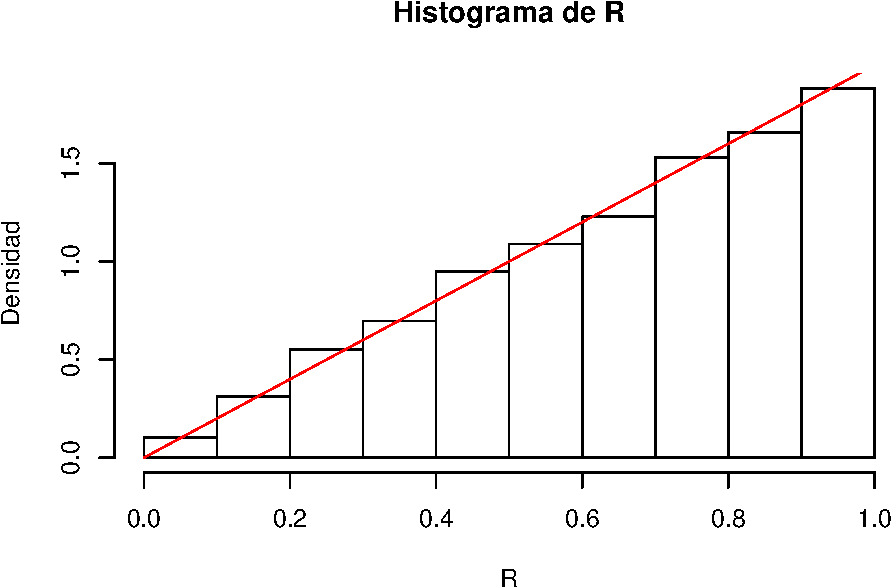
\includegraphics[width=0.75\linewidth]{notebook_simulaciones_files/figure-latex/unnamed-chunk-1-1}

Gracias a la simulación, es posible apreciar que los datos de \(R\)
simulados a partir de dos variables uniformes, se ajustan a la
distribución teórica. La línea de color rojo es la teórica y la de color
negro es la de la simulación.

\section{Ejercicio 12.11}\label{ejercicio-12.11}

Sean \((X, Y)\) normales independientes, ambas con media \(\mu=0\) y
varianza \(\sigma^2\). Sea

\[
Z = \sqrt{X^2 + Y^2} \quad \text{y}\quad W=Arctan\left(\frac{X}{Y}\right), \quad\quad\quad-\frac{\pi}{2}<W\leq\frac{\pi}{2}.
\] Demuestre que \(Z\) tiene distribución Rayleigh, que \(W\) es
uniforme sobre \(\left(-\frac{\pi}{2},\frac{\pi}{2} \right)\) y que
\(Z\) y \(W\) son independientes.

\newpage

\subsection{\texorpdfstring{\emph{Demostración:}}{Demostración:}}\label{demostracion-1}

Sea
\(g(x,y)=\left(\sqrt{x^2+y^2}\right), \tan^{-1}\left(\frac{x}{y}\right)\)

En este caso las inversas serían \(g_1^{-1}(z,w)=(z\sin w,z\cos w)\) y
\(g_2^{-1}(z,w)=(z\sin w,-z\cos w)\) puesto que \(g\) no es inyectiva.
Sus correspondientes jacobianos serían:

\begin{equation}
\left| J_{g_1^{-1}}  \right|
=\left| \det 
\begin{bmatrix} 
\sin w &  z\cos w \\
\cos w &  -z\sin w \\
\end{bmatrix}  \right|
=|-z|=z
\end{equation}

\begin{equation}
\left| J_{g_2^{-1}}  \right|
=\left| \det 
\begin{bmatrix} 
\sin w &  z\cos w \\
-\cos w &  z\sin w \\
\end{bmatrix}  \right|
=|z|=z
\end{equation}

De esta forma, se tiene que:

\begin{equation}
\begin{split}
f_{(Z,W)}(z,w) \quad &= \quad \left( \frac{1}{2\pi\sigma^2}e^{\frac{-z^2}{2\sigma^2}}z + \frac{1}{2\pi\sigma^2}e^{\frac{-z^2}{2\sigma^2}}z \right) I_{\left(-\frac{\pi}{2},\frac{\pi}{2}\right)}(w) I_{(0,\infty)}(z)\\
&=\quad \frac{1}{\pi}I_{\left(-\frac{\pi}{2},\frac{\pi}{2}\right)}(w)
\cdot\frac{z}{\sigma^2}e^{\frac{-z^2}{2\sigma^2}} I_{(0,\infty)}(z)
\end{split}
\end{equation}

Lo que demuestra que \(Z\) tiene distribución Rayleigh(\(\sigma^2\)),
\(W\) es uniforme sobre el intervalo
\(\left( -\frac{\pi}{2},\frac{\pi}{2} \right)\) y que \(Z\) y \(W\) son
independientes.

\subsection{\texorpdfstring{\emph{Simulación:}}{Simulación:}}\label{simulacion-1}

Sean \(X\) y \(Y\) dos variables aleatorias independientes con
distribución normal con media \(\mu=0\) y varianza \(\sigma^2=4\)

\begin{Shaded}
\begin{Highlighting}[]
\KeywordTok{library}\NormalTok{(VGAM)}

\KeywordTok{set.seed}\NormalTok{(}\DecValTok{163053}\NormalTok{)}

\NormalTok{X<-}\KeywordTok{rnorm}\NormalTok{(}\DecValTok{10000}\NormalTok{,}\DecValTok{0}\NormalTok{,}\DecValTok{2}\NormalTok{)}
\NormalTok{Y<-}\KeywordTok{rnorm}\NormalTok{(}\DecValTok{10000}\NormalTok{,}\DecValTok{0}\NormalTok{,}\DecValTok{2}\NormalTok{)}
\NormalTok{Z<-}\KeywordTok{sqrt}\NormalTok{(X}\OperatorTok{^}\DecValTok{2}\OperatorTok{+}\NormalTok{Y}\OperatorTok{^}\DecValTok{2}\NormalTok{)}
\end{Highlighting}
\end{Shaded}

A continuación se simulan datos de una distribución Rayleigh con
\(\sigma=2\):

\begin{Shaded}
\begin{Highlighting}[]
\NormalTok{R<-}\KeywordTok{rrayleigh}\NormalTok{(}\DecValTok{10000}\NormalTok{,}\DecValTok{2}\NormalTok{)}
\end{Highlighting}
\end{Shaded}

Al comparar los dos histogramas de los datos simulados a partir de \(X\)
y \(Y\) con los de \(Z\):

\begin{Shaded}
\begin{Highlighting}[]
\KeywordTok{par}\NormalTok{(}\DataTypeTok{mfrow=}\KeywordTok{c}\NormalTok{(}\DecValTok{1}\NormalTok{,}\DecValTok{2}\NormalTok{))}
\KeywordTok{hist}\NormalTok{(Z,}\DataTypeTok{freq =}\NormalTok{ F,}\DataTypeTok{breaks =} \DecValTok{10}\NormalTok{, }\DataTypeTok{main =} \StringTok{"Histograma de Z"}\NormalTok{, }\DataTypeTok{xlab=}\StringTok{"Z"}\NormalTok{, }\DataTypeTok{ylab =} \StringTok{"Densidad"}\NormalTok{)}


\KeywordTok{hist}\NormalTok{(R,}\DataTypeTok{freq =}\NormalTok{ F,}\DataTypeTok{breaks =} \DecValTok{10}\NormalTok{, }\DataTypeTok{main =} \StringTok{"Histograma de R"}\NormalTok{, }\DataTypeTok{xlab=}\StringTok{"R"}\NormalTok{, }\DataTypeTok{ylab =} \StringTok{"Densidad"}\NormalTok{)}
\end{Highlighting}
\end{Shaded}

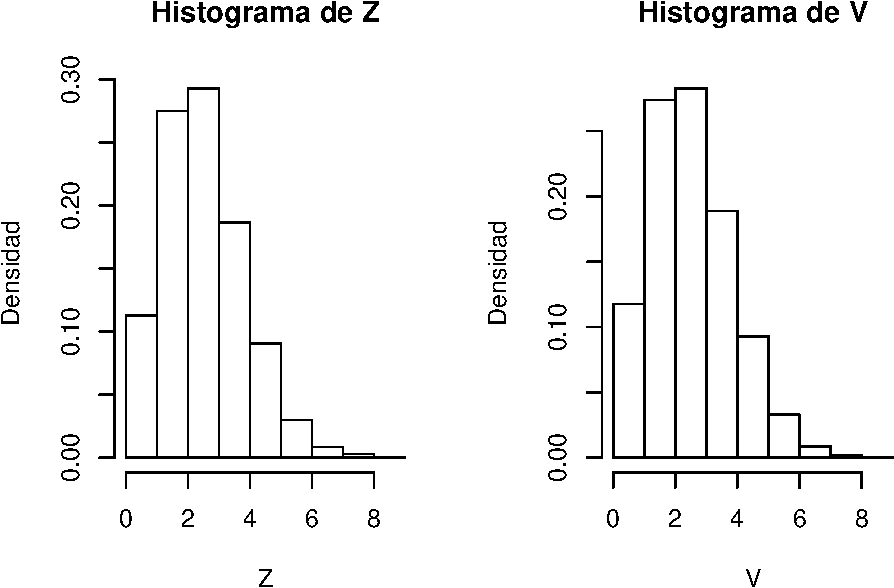
\includegraphics[width=0.8\linewidth]{notebook_simulaciones_files/figure-latex/unnamed-chunk-4-1}

Puede verse que los dos histogramas son similares, es decir, que tanto
los datos simulados (\(Z\)) a partir de dos normales como los obtenidos
(\(R\)) son equivalentes. Si se comparan con la función de densidad
teórica:

\begin{Shaded}
\begin{Highlighting}[]
\NormalTok{rayleigh<-}\ControlFlowTok{function}\NormalTok{(x,y)\{}
\NormalTok{  (x}\OperatorTok{/}\NormalTok{y}\OperatorTok{^}\DecValTok{2}\NormalTok{)}\OperatorTok{*}\KeywordTok{exp}\NormalTok{((}\OperatorTok{-}\NormalTok{x}\OperatorTok{^}\DecValTok{2}\NormalTok{)}\OperatorTok{/}\NormalTok{(}\DecValTok{2}\OperatorTok{*}\NormalTok{y}\OperatorTok{^}\DecValTok{2}\NormalTok{))}
\NormalTok{\}}

\KeywordTok{par}\NormalTok{(}\DataTypeTok{mfrow=}\KeywordTok{c}\NormalTok{(}\DecValTok{1}\NormalTok{,}\DecValTok{1}\NormalTok{))}
\KeywordTok{hist}\NormalTok{(Z,}\DataTypeTok{freq =}\NormalTok{ F,}\DataTypeTok{breaks =} \DecValTok{10}\NormalTok{,}\DataTypeTok{ylim =} \KeywordTok{c}\NormalTok{(}\DecValTok{0}\NormalTok{,}\FloatTok{0.35}\NormalTok{), }
     \DataTypeTok{main =} \StringTok{"Histograma de Z"}\NormalTok{, }\DataTypeTok{xlab=}\StringTok{"Z"}\NormalTok{, }\DataTypeTok{ylab =} \StringTok{"Densidad"}\NormalTok{)}
\KeywordTok{curve}\NormalTok{(}\KeywordTok{rayleigh}\NormalTok{(x,}\DecValTok{2}\NormalTok{),}\DataTypeTok{from =} \DecValTok{0}\NormalTok{,}\DataTypeTok{to =} \DecValTok{8}\NormalTok{,}\DataTypeTok{add =}\NormalTok{ T,}\DataTypeTok{col=}\DecValTok{2}\NormalTok{)}
\KeywordTok{lines}\NormalTok{(}\KeywordTok{density}\NormalTok{(Z))}
\end{Highlighting}
\end{Shaded}

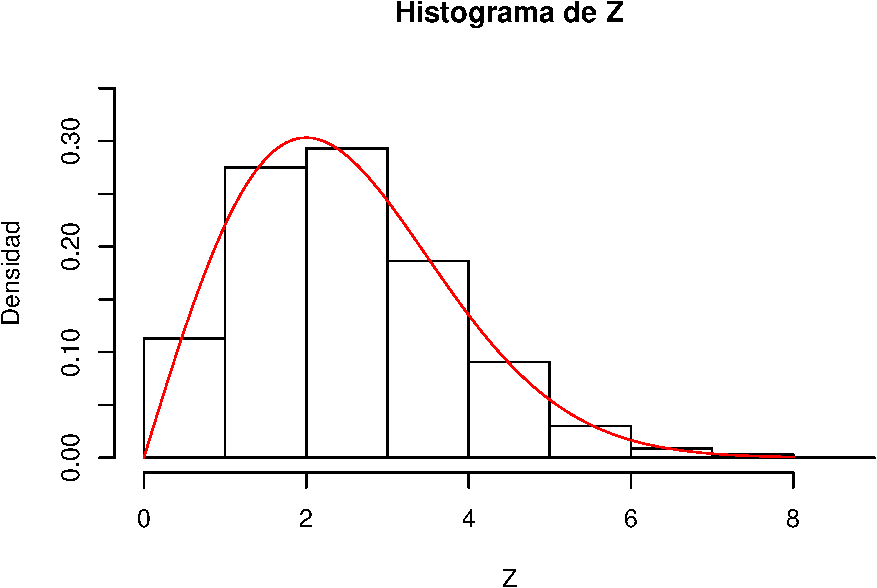
\includegraphics[width=0.8\linewidth]{notebook_simulaciones_files/figure-latex/unnamed-chunk-5-1}

\begin{Shaded}
\begin{Highlighting}[]
\KeywordTok{ks.test}\NormalTok{(Z,prayleigh,}\DecValTok{2}\NormalTok{)}
\end{Highlighting}
\end{Shaded}

\begin{verbatim}
## 
##  One-sample Kolmogorov-Smirnov test
## 
## data:  Z
## D = 0.0091383, p-value = 0.3739
## alternative hypothesis: two-sided
\end{verbatim}

\begin{Shaded}
\begin{Highlighting}[]
\NormalTok{test <-}\StringTok{ }\KeywordTok{ks.test}\NormalTok{(Z,prayleigh,}\DecValTok{2}\NormalTok{)}
\end{Highlighting}
\end{Shaded}

De esta forma, es posible confirmar que los datos de la distribución
Rayleigh simulados a partir de dos normales coninciden con la función de
densidad de una distribución Rayleigh. La línea de color rojo es la
teórica y la de color negro es la de la simulación. Igualmente, se
utiliza el test de Kolmogorov-Smirnov, con un \(\alpha=0.05\) cuya
hipótesis nula afirma que los datos siguen la distribución deseada, en
este caso Rayleigh. Como puede verse, el p-valor 0.3739197 permite no
rechazar la hipótesis nula indicada, de tal suerte que la prueba
confirma que los datos siguen una distribución Rayleigh.

Ahora, sean \(X\) y \(Y\) dos variables aleatorias normales
independientes con media \(\mu=0\) y varianza \(\sigma^2=4\)

\begin{Shaded}
\begin{Highlighting}[]
\KeywordTok{set.seed}\NormalTok{(}\DecValTok{163053}\NormalTok{)}

\NormalTok{X<-}\KeywordTok{rnorm}\NormalTok{(}\DecValTok{10000}\NormalTok{,}\DecValTok{0}\NormalTok{,}\DecValTok{2}\NormalTok{)}
\NormalTok{Y<-}\KeywordTok{rnorm}\NormalTok{(}\DecValTok{10000}\NormalTok{,}\DecValTok{0}\NormalTok{,}\DecValTok{2}\NormalTok{)}

\NormalTok{U<-X}\OperatorTok{/}\NormalTok{Y}
\NormalTok{W<-}\KeywordTok{atan}\NormalTok{(U)}
\end{Highlighting}
\end{Shaded}

Al simular datos \(Z\) de una distribución uniforme \(U(-\pi/2,\pi/2)\),
se tiene:.

\begin{Shaded}
\begin{Highlighting}[]
\NormalTok{Z<-}\KeywordTok{runif}\NormalTok{(}\DecValTok{10000}\NormalTok{,}\OperatorTok{-}\NormalTok{pi}\OperatorTok{/}\DecValTok{2}\NormalTok{,pi}\OperatorTok{/}\DecValTok{2}\NormalTok{)}
\end{Highlighting}
\end{Shaded}

Al comparar los dos histogramas de los datos simulados a partir \(X\) y
\(Y\) y los de \(Z\):

\begin{Shaded}
\begin{Highlighting}[]
\KeywordTok{par}\NormalTok{(}\DataTypeTok{mfrow=}\KeywordTok{c}\NormalTok{(}\DecValTok{1}\NormalTok{,}\DecValTok{2}\NormalTok{))}
\KeywordTok{hist}\NormalTok{(W,}\DataTypeTok{freq =} \OtherTok{FALSE}\NormalTok{, }\DataTypeTok{main =} \StringTok{"Histograma de W"}\NormalTok{, }\DataTypeTok{xlab=}\StringTok{"W"}\NormalTok{, }\DataTypeTok{ylab =} \StringTok{"Densidad"}\NormalTok{)}
\KeywordTok{hist}\NormalTok{(Z,}\DataTypeTok{freq =} \OtherTok{FALSE}\NormalTok{, }\DataTypeTok{main =} \StringTok{"Histograma de Z"}\NormalTok{, }\DataTypeTok{xlab=}\StringTok{"Z"}\NormalTok{, }\DataTypeTok{ylab =} \StringTok{"Densidad"}\NormalTok{)}
\end{Highlighting}
\end{Shaded}

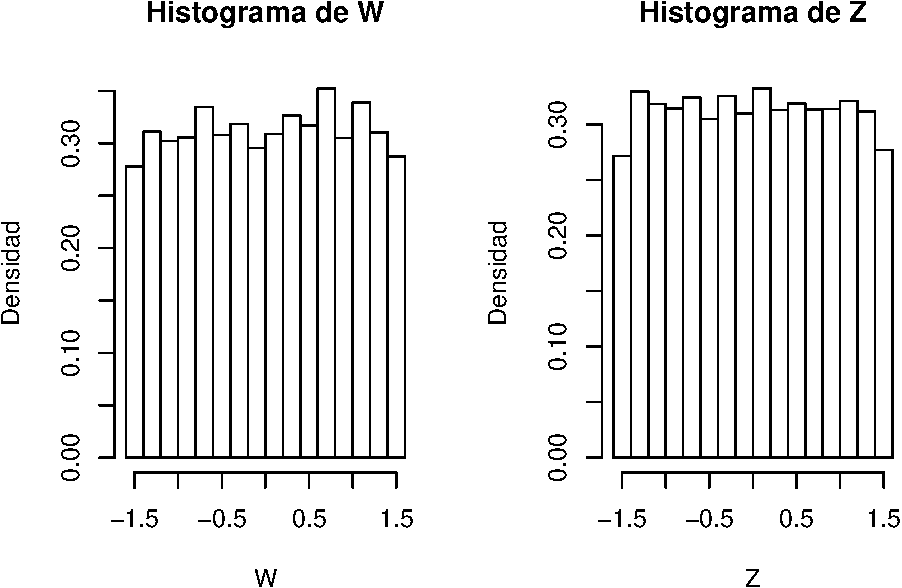
\includegraphics[width=0.75\linewidth]{notebook_simulaciones_files/figure-latex/unnamed-chunk-8-1}

Se observa que los dos histogramas son similares, es decir, que tanto
los simulados \(W\) a partir de dos normales y los obtenidos \((Z)\) son
equivalentes. Al comparar con la función de densidad teórica:

\begin{Shaded}
\begin{Highlighting}[]
\NormalTok{unifor<-}\ControlFlowTok{function}\NormalTok{(x,y,z)\{}
  \ControlFlowTok{if}\NormalTok{(x}\OperatorTok{>=}\NormalTok{y}\OperatorTok{&}\NormalTok{x}\OperatorTok{<=}\NormalTok{z)\{}\DecValTok{1}\OperatorTok{/}\NormalTok{(z}\OperatorTok{-}\NormalTok{y)\}}
  \ControlFlowTok{else}\NormalTok{\{}\DecValTok{0}\NormalTok{\}}
\NormalTok{\}}

\NormalTok{unif<-}\KeywordTok{Vectorize}\NormalTok{(unifor)}

\KeywordTok{par}\NormalTok{(}\DataTypeTok{mfrow=}\KeywordTok{c}\NormalTok{(}\DecValTok{1}\NormalTok{,}\DecValTok{1}\NormalTok{))}
\KeywordTok{hist}\NormalTok{(W,}\DataTypeTok{freq =} \OtherTok{FALSE}\NormalTok{, }\DataTypeTok{main =} \StringTok{"Histograma de W"}\NormalTok{, }\DataTypeTok{xlab=}\StringTok{"W"}\NormalTok{, }\DataTypeTok{ylab =} \StringTok{"Densidad"}\NormalTok{)}
\KeywordTok{curve}\NormalTok{(}\KeywordTok{unif}\NormalTok{(x,}\OperatorTok{-}\NormalTok{pi}\OperatorTok{/}\DecValTok{2}\NormalTok{,pi}\OperatorTok{/}\DecValTok{2}\NormalTok{),}\DataTypeTok{add =}\NormalTok{ T,}\DataTypeTok{col=}\DecValTok{2}\NormalTok{)}
\end{Highlighting}
\end{Shaded}

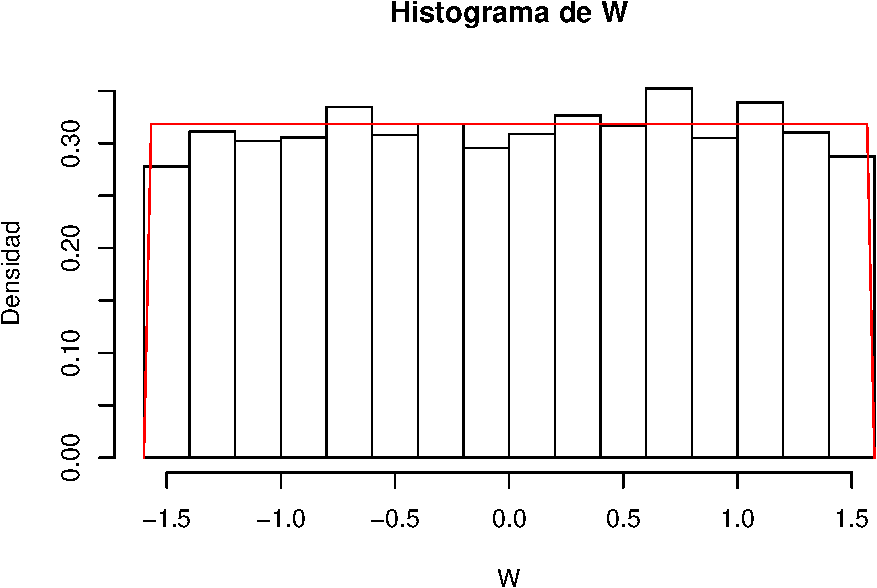
\includegraphics[width=0.7\linewidth]{notebook_simulaciones_files/figure-latex/unnamed-chunk-9-1}

\begin{Shaded}
\begin{Highlighting}[]
\KeywordTok{ks.test}\NormalTok{(W,punif,}\OperatorTok{-}\NormalTok{pi}\OperatorTok{/}\DecValTok{2}\NormalTok{,pi}\OperatorTok{/}\DecValTok{2}\NormalTok{)}
\end{Highlighting}
\end{Shaded}

\begin{verbatim}
## 
##  One-sample Kolmogorov-Smirnov test
## 
## data:  W
## D = 0.012268, p-value = 0.09855
## alternative hypothesis: two-sided
\end{verbatim}

\begin{Shaded}
\begin{Highlighting}[]
\NormalTok{test <-}\StringTok{ }\KeywordTok{ks.test}\NormalTok{(W,punif,}\OperatorTok{-}\NormalTok{pi}\OperatorTok{/}\DecValTok{2}\NormalTok{,pi}\OperatorTok{/}\DecValTok{2}\NormalTok{)}
\end{Highlighting}
\end{Shaded}

Se confirma que los datos de la distribución uniforme entre \(-\pi/2\) y
\(\pi/2\) simulados a partir de dos normales coninciden con la función
de densidad de la una distribución uniforme. La línea de color rojo es
la teórica. Igualmente, se utiliza el test de Kolmogorov-Smirnov, con un
\(\alpha=0.05\) cuya hipótesis nula afirma que los datos siguen la
distribución deseada. En este caso, el p-valor 0.0985464 permite no
rechazar la hipótesis nula indicada y gracias a esta prueba, ratificar
que los datos siguen distribución uniforme.

\newpage

\section{Ejercicio 12.15}\label{ejercicio-12.15}

(\emph{Simulación de variables aleatorias normales}) Sean \(U\), \(V\)
dos variables aleatorias uniformes independientes sobre \((0,1)\). Sean
\(\theta=2\pi U\) y \(S=-\ln(V)\).

(\emph{Pista:} Para la parte \emph{(a)} recuerde que una exponencial es
un caso especial de una distribución Gamma: de hecho, esto es
\(\chi_2^2\). Para la parte (b) invierta el procedimiento del esjericio
12.11).

\emph{Observación:} El ejercicio 12.15 es conocido como el método
Box-Muller para simular variables aleatorias normales.

\begin{enumerate}
\def\labelenumi{\alph{enumi}.}
\tightlist
\item
  Demuestre que \(S\) tiene distribución exponencial, y que
  \(R =\sqrt{2S}\) tiene distribución Rayleigh.
\end{enumerate}

\subsection{\texorpdfstring{\emph{Demostración:}}{Demostración:}}\label{demostracion-2}

Sea \(V \sim U(0,1)\) y \(S=-\ln(V)\), luego

\begin{equation}
s=g(v)=-\ln(v)\Rightarrow v=h(s)=e^{-s}
\end{equation}

Así,

\begin{equation}
|h'(s)|=\left| \frac{dh(s)}{ds}  \right|=\left| -e^{-s}  \right|=e^{-s}
\end{equation}

Como

\begin{equation}
f_V(v)=1I_{(0,1)} \quad f_S(s)=f_V(e^{-s})\cdot \left| \frac{dv}{ds}  \right|=1\cdot e^{-s}=e^{-s}
\end{equation}

De tal suerte que puede concluirse que \(S \sim Exp(1)\)

Ahora,

\begin{equation}
\begin{split}
R=\sqrt{2S}=\sqrt{-2\ln(V)}\\
R=h(v)=\sqrt{-2\ln(V)}
\end{split}
\end{equation}

Luego,

\begin{equation}
\begin{split}
r =g(v)= \sqrt{-2\ln(v)}\\
r^2 = -2\ln(v)\\
-\frac{r^2}{2}=\ln(v)\\
v=h(r)=e^{-\frac{r^2}{2}}
\end{split}
\end{equation}

De esta forma, \[
|h'(s)|=\left| \frac{dh(s)}{ds}  \right|=\left| =-r\cdot e^{-\frac{r^2}{2}}  \right|=r\cdot e^{-\frac{r^2}{2}} 
\] \newpage
Entonces,

\[
f_V(v)=1I_{(0,1)} \quad f_R(r)=f_V(e^{-\frac{r^2}{2}})\cdot \left| \frac{dv}{ds}  \right|=1\cdot r e^{-\frac{r^2}{2}}=r\cdot e^{-\frac{r^2}{2}}
\]

Que claramente se refiere a una variable aleatoria \(R\sim Rayleigh(1)\)

\subsection{\texorpdfstring{\emph{Simulación:}}{Simulación:}}\label{simulacion-2}

Sea \(V\) una variable aleatoria con distribución uniforme en \((0,1)\)

\begin{Shaded}
\begin{Highlighting}[]
\KeywordTok{set.seed}\NormalTok{(}\DecValTok{163053}\NormalTok{)}
\NormalTok{V<-}\KeywordTok{runif}\NormalTok{(}\DecValTok{10000}\NormalTok{)}
\NormalTok{S<-}\OperatorTok{-}\KeywordTok{log}\NormalTok{(V)}
\NormalTok{R<-}\KeywordTok{sqrt}\NormalTok{(}\DecValTok{2}\OperatorTok{*}\NormalTok{S)}

\KeywordTok{hist}\NormalTok{(S,}\DataTypeTok{freq =} \OtherTok{FALSE}\NormalTok{, }\DataTypeTok{main =} \StringTok{"Histograma de S"}\NormalTok{, }\DataTypeTok{xlab=}\StringTok{"S"}\NormalTok{, }\DataTypeTok{ylab =} \StringTok{"Densidad"}\NormalTok{)}
\KeywordTok{curve}\NormalTok{(}\KeywordTok{dexp}\NormalTok{(x,}\DecValTok{1}\NormalTok{),}\DataTypeTok{add=}\NormalTok{T,}\DataTypeTok{col=}\DecValTok{2}\NormalTok{)}
\KeywordTok{lines}\NormalTok{(}\KeywordTok{density}\NormalTok{(S))}
\end{Highlighting}
\end{Shaded}

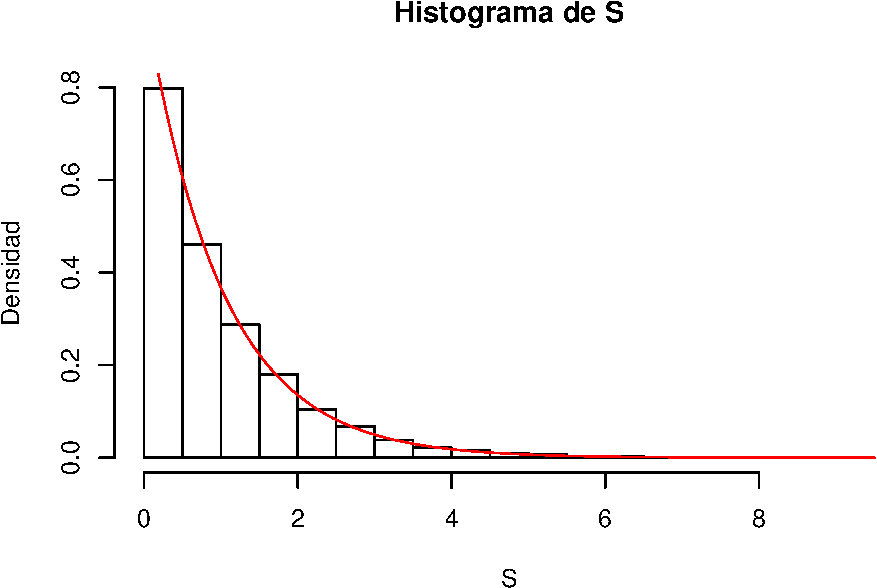
\includegraphics[width=0.63\linewidth]{notebook_simulaciones_files/figure-latex/unnamed-chunk-10-1}

\begin{Shaded}
\begin{Highlighting}[]
\KeywordTok{ks.test}\NormalTok{(S,pexp,}\DecValTok{1}\NormalTok{)}
\end{Highlighting}
\end{Shaded}

\begin{verbatim}
## 
##  One-sample Kolmogorov-Smirnov test
## 
## data:  S
## D = 0.0081251, p-value = 0.5239
## alternative hypothesis: two-sided
\end{verbatim}

\begin{Shaded}
\begin{Highlighting}[]
\NormalTok{test <-}\StringTok{ }\KeywordTok{ks.test}\NormalTok{(S,pexp,}\DecValTok{1}\NormalTok{)}
\end{Highlighting}
\end{Shaded}

Se observa que los datos de \(S\) simulados a partir de una distribución
uniforme, se ajusta a una distribución exponencial con parámetro 1. Una
vez más, se utiliza el test de Kolmogorov-Smirnov, con un
\(\alpha=0.05\) cuya hipótesis nula afirma que los datos siguen la
distribución deseada. En este caso, el p-valor 0.5239289 permite no
rechazar la hipótesis nula indicada y gracias a esta prueba, ratificar
que los datos siguen distribución exponencial.

\newpage

Por otra parte, los datos simulados de \(R\)

\begin{Shaded}
\begin{Highlighting}[]
\KeywordTok{hist}\NormalTok{(R,}\DataTypeTok{freq =} \OtherTok{FALSE}\NormalTok{, }\DataTypeTok{main =} \StringTok{"Histograma de R"}\NormalTok{, }\DataTypeTok{xlab=}\StringTok{"R"}\NormalTok{, }\DataTypeTok{ylab =} \StringTok{"Densidad"}\NormalTok{)}
\KeywordTok{curve}\NormalTok{(}\KeywordTok{drayleigh}\NormalTok{(x,}\DataTypeTok{scale =} \DecValTok{1}\NormalTok{),}\DataTypeTok{add=}\NormalTok{T,}\DataTypeTok{col=}\DecValTok{2}\NormalTok{)}
\KeywordTok{lines}\NormalTok{(}\KeywordTok{density}\NormalTok{(R))}
\end{Highlighting}
\end{Shaded}

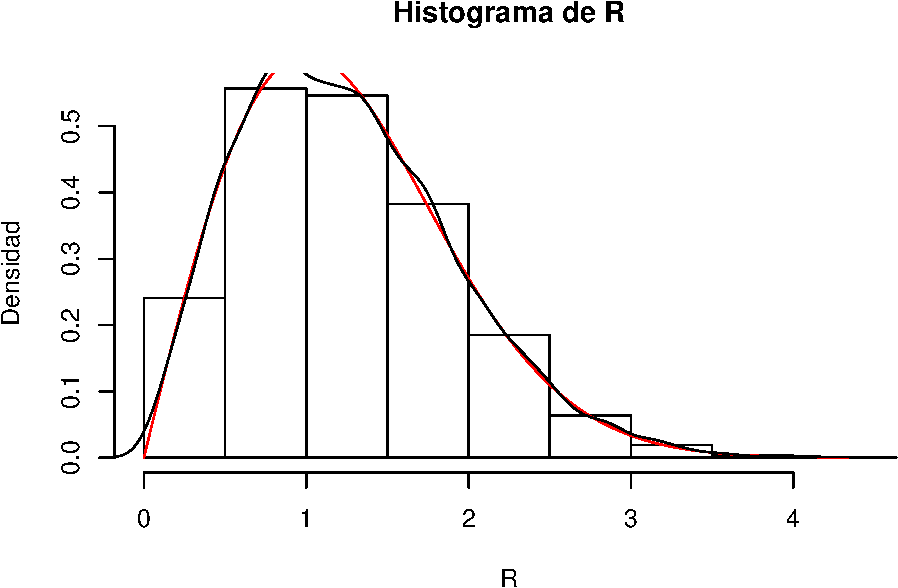
\includegraphics[width=0.63\linewidth]{notebook_simulaciones_files/figure-latex/unnamed-chunk-11-1}

\begin{Shaded}
\begin{Highlighting}[]
\KeywordTok{ks.test}\NormalTok{(R,prayleigh,}\DecValTok{2}\NormalTok{)}
\end{Highlighting}
\end{Shaded}

\begin{verbatim}
## 
##  One-sample Kolmogorov-Smirnov test
## 
## data:  R
## D = 0.47318, p-value < 2.2e-16
## alternative hypothesis: two-sided
\end{verbatim}

\begin{Shaded}
\begin{Highlighting}[]
\NormalTok{test <-}\StringTok{ }\KeywordTok{ks.test}\NormalTok{(R,prayleigh,}\DecValTok{2}\NormalTok{)}
\end{Highlighting}
\end{Shaded}

Se observa que los datos de \(R\) simulados a partir de una distribución
exponencial de parámetro 1, se ajusta a una distribución Rayleigh con
parámetro 1. Una vez más, se utiliza el test de Kolmogorov-Smirnov, con
un \(\alpha=0.05\) cuya hipótesis nula afirma que los datos siguen la
distribución deseada. En este caso, el p-valor 0 permite no rechazar la
hipótesis nula indicada y gracias a esta prueba, ratificar que los datos
siguen distribución Rayleigh.

\begin{enumerate}
\def\labelenumi{\alph{enumi}.}
\setcounter{enumi}{1}
\tightlist
\item
  Sean \(X=R \cos\theta\), \(Y=R\sin\theta\). Demuestre que \(X\) y
  \(Y\) son normales independientes.
\end{enumerate}

\subsection{\texorpdfstring{\emph{Demostración:}}{Demostración:}}\label{demostracion-3}

Se sabe que \(X=\sqrt{-2\ln(V)}\cos(2\pi U)\) y
\(Y=\sqrt{-2\ln(V)}\sin(2\pi U)\).

Así,
\(g(u,v)=(\sqrt{-2\ln(v)}\cos(2\pi u),\sqrt{-2\ln(v)}\sin(2\pi u))\)

A continuación se calculan la inversa de \(g\):

\begin{equation}
\frac{Y}{X}=\frac{\sqrt{-2\ln(v)}\cos(2\pi u)}{\sqrt{-2\ln(v)}\sin(2\pi u)}
=\tan(2 \pi u) \Rightarrow u=\frac{1}{2 \pi}\tan^{-1}\left( \frac{y}{x}  \right)
\end{equation}

Por otra parte,

\begin{equation}
\begin{split}
X^2+Y^2&=(\sqrt{-2\ln(v)}\cos(2\pi u)^2+(\sqrt{-2\ln(v)}\sin(2\pi u)^2\\
&= (-2\ln(v)\cos^2(2\pi u))+(-2\ln(v)\sin^2(2\pi u)\\
&= -2\ln(v)(\cos^2(2\pi u)+\sin^2(2\pi u)\\
&= -2\ln(v)
\end{split}
\end{equation}

Así,

\begin{equation}
v = e^{-\frac{x^2+y^2}{2}}
\end{equation}

De esta forma,
\(g^{-1}(x,y)= \left(\frac{1}{2 \pi}\tan^{-1}\left( \frac{y}{x} \right),e^{-\frac{x^2+y^2}{2}}\right)\)

El cálculo del jacobiano se presenta a continuación:

\begin{equation}
\begin{split}
\left| J_{g^{-1}}  \right|
&=\left| \det 
\begin{bmatrix} 
\frac{y}{2\pi(x^2+y^2)} &  -\frac{x}{2\pi(x^2+y^2)} \\
-x\cdot e^{-\frac{x^2+y^2}{2}} &  -y\cdot e^{-\frac{x^2+y^2}{2}} \\
\end{bmatrix}  \right|\\
&=
\left|
\frac{-y^2\cdot e^{-\frac{x^2+y^2}{2}}}{2\pi(x^2+y^2)}-
\frac{-x^2\cdot e^{-\frac{x^2+y^2}{2}}}{2\pi(x^2+y^2)}
\right|\\
&=
\left|
\frac{-y^2\cdot e^{-\frac{x^2+y^2}{2}}-x^2\cdot e^{-\frac{x^2+y^2}{2}}}{2\pi(x^2+y^2)}
\right|\\
&=
\left|
\frac{-e^{-\frac{x^2+y^2}{2}}(x^2+y^2)}{2\pi(x^2+y^2)}
\right|\\
&=
\frac{1}{2\pi}e^{-\frac{x^2+y^2}{2}}
\end{split}
\end{equation}

De esta forma, la densidad conjunta de \(X\) y \(Y\) es:

\begin{equation}
f_{X,Y}=\frac{1}{2\pi}e^{-\frac{x^2+y^2}{2}}=\frac{1}{\sqrt{2\pi}}e^{-\frac{x^2}{2}} \cdot \frac{1}{\sqrt{2\pi}}e^{-\frac{y^2}{2}}=f(x)f(y)
\end{equation}

Lo que demuestra que \(X\) y \(Y\) se distribuyen normales estándar y
además son independientes.

\subsection{\texorpdfstring{\emph{Simulación:}}{Simulación:}}\label{simulacion-3}

Sean \(U\) y \(V\) variables aleatorias uniformes en \((0,1)\)

\begin{Shaded}
\begin{Highlighting}[]
\NormalTok{n =}\StringTok{ }\DecValTok{200}
\NormalTok{U=}\KeywordTok{runif}\NormalTok{(n)}
\NormalTok{V=}\KeywordTok{runif}\NormalTok{(n)}
\NormalTok{X=}\KeywordTok{sqrt}\NormalTok{(}\OperatorTok{-}\DecValTok{2}\OperatorTok{*}\KeywordTok{log}\NormalTok{(U))}\OperatorTok{*}\KeywordTok{cos}\NormalTok{(}\DecValTok{2}\OperatorTok{*}\NormalTok{pi}\OperatorTok{*}\NormalTok{V)}
\NormalTok{Y=}\KeywordTok{sqrt}\NormalTok{(}\OperatorTok{-}\DecValTok{2}\OperatorTok{*}\KeywordTok{log}\NormalTok{(V))}\OperatorTok{*}\KeywordTok{cos}\NormalTok{(}\DecValTok{2}\OperatorTok{*}\NormalTok{pi}\OperatorTok{*}\NormalTok{U)}
\NormalTok{x=}\KeywordTok{seq}\NormalTok{(}\OperatorTok{-}\DecValTok{3}\NormalTok{,}\DecValTok{3}\NormalTok{,}\DataTypeTok{by=}\NormalTok{.}\DecValTok{01}\NormalTok{)}
\KeywordTok{par}\NormalTok{(}\DataTypeTok{mfrow=}\KeywordTok{c}\NormalTok{(}\DecValTok{1}\NormalTok{,}\DecValTok{2}\NormalTok{))}
\KeywordTok{hist}\NormalTok{(X,}\DataTypeTok{freq =}\NormalTok{ F);}\KeywordTok{lines}\NormalTok{(x,}\KeywordTok{dnorm}\NormalTok{(x,}\KeywordTok{mean}\NormalTok{(X),}\KeywordTok{sd}\NormalTok{(X)))}
\KeywordTok{hist}\NormalTok{(Y,}\DataTypeTok{freq =}\NormalTok{ F);}\KeywordTok{lines}\NormalTok{(x,}\KeywordTok{dnorm}\NormalTok{(x,}\KeywordTok{mean}\NormalTok{(Y),}\KeywordTok{sd}\NormalTok{(Y)))}
\end{Highlighting}
\end{Shaded}

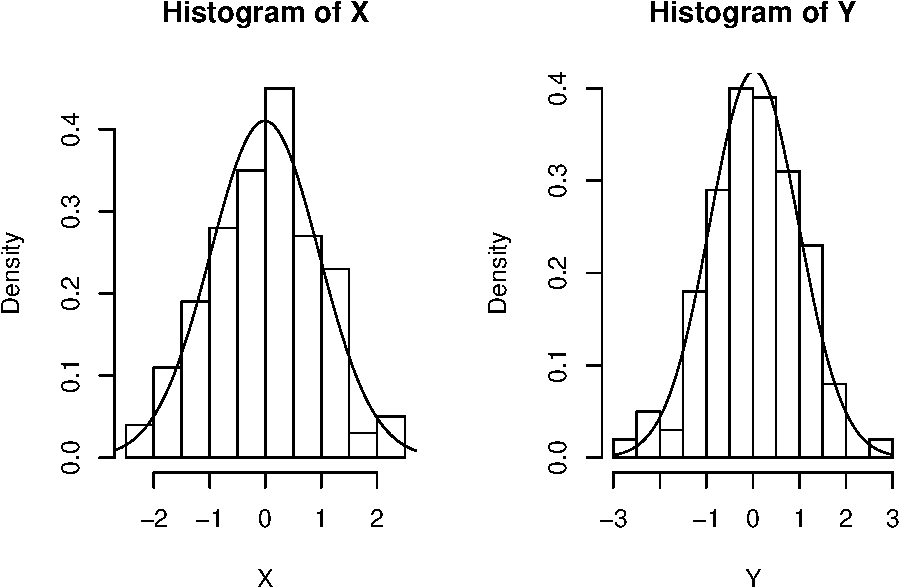
\includegraphics{notebook_simulaciones_files/figure-latex/unnamed-chunk-12-1.pdf}

Puede observarse que las variables simuladas de \(X\) y \(Y\),
corresponden a variables normales con media 0 y varianza 4.

\begin{Shaded}
\begin{Highlighting}[]
\KeywordTok{ks.test}\NormalTok{(X,pnorm) }
\end{Highlighting}
\end{Shaded}

\begin{verbatim}
## 
##  One-sample Kolmogorov-Smirnov test
## 
## data:  X
## D = 0.034158, p-value = 0.9738
## alternative hypothesis: two-sided
\end{verbatim}

\begin{Shaded}
\begin{Highlighting}[]
\NormalTok{test1 <-}\StringTok{ }\KeywordTok{ks.test}\NormalTok{(X,pnorm)}
\KeywordTok{ks.test}\NormalTok{(Y,pnorm)}
\end{Highlighting}
\end{Shaded}

\begin{verbatim}
## 
##  One-sample Kolmogorov-Smirnov test
## 
## data:  Y
## D = 0.049467, p-value = 0.712
## alternative hypothesis: two-sided
\end{verbatim}

\begin{Shaded}
\begin{Highlighting}[]
\NormalTok{test2 <-}\StringTok{ }\KeywordTok{ks.test}\NormalTok{(Y,pnorm)}
\end{Highlighting}
\end{Shaded}

Se utiliza el test de Kolmogorov-Smirnov, con un \(\alpha=0.05\) cuya
hipótesis nula afirma que los datos siguen la distribución deseada. En
este caso, los p-valores 0.9737566 y 0.7119575 permiten no rechazar la
hipótesis nula indicada y gracias a esta prueba, ratificar que los datos
siguen distribución Normal para cada una de las variables \(X\) y \(Y\).


\end{document}
